\documentclass[a4paper,10pt]{article}
\usepackage[utf8]{inputenc}
\usepackage[left=2.5cm, top=2.5cm, right=2.5cm, bottom=2.5cm]{geometry}
\usepackage[spanish]{babel}
\usepackage{enumitem}
\usepackage{hyperref}


\begin{document}

% Carátula
\begin{titlepage}
    \centering
    \vspace*{3cm}
    {\Large {Introducción a los Sistemas Distribuidos (75.43)}}\\[0.5cm]
    {\Large{TP Nº1: File Transfer}}\\[1cm]
    {\large Esteban Carisimo y Juan Ignacio Lopez Pecora}\\[0.5cm]
    {\large Facultad de Ingeniería, Universidad de Buenos Aires (75.43)}\\[2cm]

    {\large \textbf{Integrantes:}}\\[0.5cm]
    {\large Daniel Agustin Marianetti - 106256}\\
    {\large Lautaro Leonel Pedrozo - 110146}\\
    {\large Patricio Perrone - 98230}\\
    {\large Ezequiel Lazarte - 108063}\\[3cm]

    {\large Fecha de entrega: 8 de mayo de 2025}
\end{titlepage}

% Índice
\tableofcontents
\newpage

\section{Introducción}
El presente trabajo práctico tiene como objetivo fundamental la creación de una aplicación de red. Para alcanzar dicha finalidad, resulta indispensable comprender cómo se comunican los procesos a través de la red y analizar el modelo de servicio que la capa de transporte le ofrece a la capa de aplicación.

El objetivo específico de este trabajo es la comprensión y la puesta en práctica de los conceptos y herramientas necesarias para la implementación de un protocolo de transferencia de datos confiable (RDT). Para lograrlo, se procederá a desarrollar una aplicación de arquitectura cliente-servidor orientada a la transferencia de archivos, contemplando las operaciones de \textbf{UPLOAD} (cliente a servidor) y \textbf{DOWNLOAD} (servidor a cliente).

La implementación de esta aplicación se realizará utilizando el \textbf{lenguaje Python} y la \textbf{librería estándar de sockets}. La comunicación entre los procesos se establecerá sobre \textbf{UDP como protocolo de capa de transporte}. Para asegurar una transferencia confiable sobre UDP, se implementarán dos versiones del protocolo RDT: \textbf{Stop \& Wait} y \textbf{Selective Repeat}. Este desarrollo permitirá explorar los principios básicos de la transferencia de datos confiable y el uso de la interfaz de sockets.

\section{Hipótesis y suposiciones realizadas}
\begin{itemize}
    \item El tamaño de mensajes enviados 1024 bytes
    
    \item Explicar diseño o elección de paquetes?
    % Otros ítems de hipótesis/suposiciones irían aquí
\end{itemize}

\section{Implementación}
Explicar la arquitectura de la aplicación, los componentes principales, y cómo se utiliza la interfaz de sockets. Detallar el protocolo de red implementado para cada operación requerida.

\subsection{Mensajes/Segmentos}
Esta subsección detalla la estructura de los diferentes tipos de segmentos que se intercambian entre el cliente y el servidor para implementar el protocolo de capa de aplicación requerido.

\subsubsection{INIT}
Este segmento se utiliza para \textbf{iniciar una operación de transferencia de archivos}. 
Se define con la siguiente estructura:
\begin{itemize}
    \item \textbf{Header}: Tiene un tamaño fijo de 2 bytes.
    \begin{itemize}
        \item \textbf{Flags} (1 Byte):
        \begin{itemize}
        \item \textbf{PADDING} (5 bits)
        \item \textbf{ACK} (1 bit)
        \item \textbf{OPCODE:} Indica el tipo de operacion a realizar durante la conexión (UPLOAD o DOWNLOAD) (1 bit)
        \item \textbf{PROTOCOL:} Indica el tipo de protocolo a utilizar durante la conexión (SW o SR) (1 bit)
        \end{itemize}

        \item \textbf{File name length:} Largo en bytes del nombre de archivo (1 Byte)
    \end{itemize}
    
    \item \textbf{Payload}
    \begin{itemize}
        \item \textbf{File name:} UTF-8 string
    \end{itemize}
    
    \item \textbf{Checksum CRC32} (4 Bytes)
\end{itemize}
\begin{figure}[H]
    \centering
    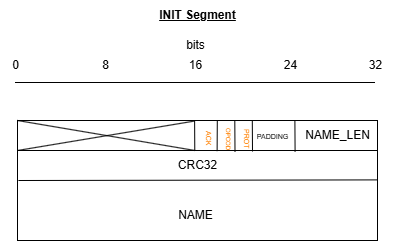
\includegraphics[width=0.5\linewidth]{init_segment.png}
    \caption{Estructura paquete INIT}
\end{figure}

\subsubsection{S\&W}
El segmento \textbf{StopAndWaitSegment} (S\&W) se utiliza para la \textbf{transferencia de datos y el control} en el protocolo RDT \textbf{Stop \& Wait}. Se define con la siguiente estructura:
\begin{itemize}
    \item \textbf{Header}: Tiene un tamaño fijo de 3 bytes.
    \begin{itemize}
        \item \textbf{Flags} (1 Byte): Contiene flags empaquetados:
        \begin{itemize}
        \item \textbf{PADDING} (5 bits)
        \item \textbf{SEQ Num:} Número de secuencia (1 bit, alternando entre 0 y 1).
        \item \textbf{ACK:} (1 bit, alternando entre 0 y 1).
        \item \textbf{EOF Num:} Indicador de fin de archivo (1 bit).
        \end{itemize}
        \item \textbf{Payload Length} (2 Bytes): Longitud en bytes del campo `payload`.
    \end{itemize}
    \item \textbf{Payload} (0 - 1017 Bytes)
    \item \textbf{Checksum CRC32} (4 Bytes)
\end{itemize}
El tamaño mínimo total de un segmento S\&W serializado (sin payload) es de 1 (header) + 2 (len payload) + 0 (payload) + 4 (CRC) = 7 bytes.
\begin{figure}[H]
    \centering
    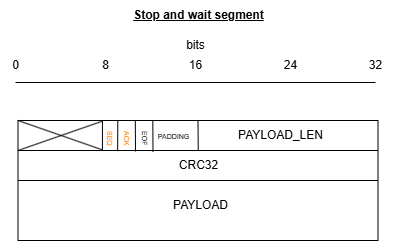
\includegraphics[width=0.5\linewidth]{sw_segment.png}
    \caption{Estructura paquete STOP AND WAIT}
\end{figure}


\subsubsection{SR}
El segmento \textbf{SelectiveRepeatSegment} (SR) se destina a la \textbf{transferencia de datos y el control} en el protocolo RDT \textbf{Selective Repeat}. Se define con la siguiente estructura:
\begin{itemize}
    \item \textbf{Header}:
    \begin{itemize}
        \item \textbf{SEQ Num} (2 Bytes): Número de secuencia. Permite un espacio de numeración más amplio para la ventana deslizante.
        \item \textbf{ACK Num} (2 Bytes)
        \item \textbf{Win Size} (2 Bytes): Tamaño de la ventana del receptor.
        \item \textbf{Payload Length} (2 Bytes): Longitud en bytes del campo `payload`.
    \end{itemize}
    \item \textbf{Payload}
    
    \item \textbf{Checksum CRC32} (4 Bytes)
\end{itemize}
El tamaño mínimo total de un segmento SR serializado (sin payload) es de 2 (seq) + 2 (ack) + 2 (win) + 2 (len payload) + 0 (payload) + 4 (CRC) = 12 bytes.
\begin{figure}[H]
    \centering
    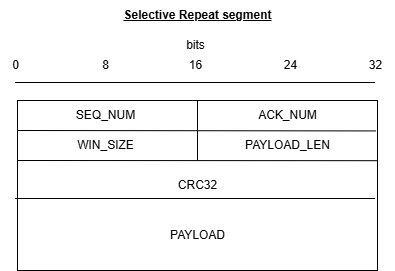
\includegraphics[width=0.5\linewidth]{sr_segment.png}
    \caption{Estructura paquete SELECTIVE REPEAT}
\end{figure}


\subsection{Handshake}
Siguiendo con la idea de formar un RDT, es necesario que el protocolo de aplicación construido permita a las partes establecer una conexión de manera que ambos sepan que del otro lado hay una parte que recibirá sus mensajes y estará también compartiendo la información. Siguiendo con el punto anterior, el mensaje INIT y su respectiva respuesta INITACK (INIT con el flag de ACK setteado en 1) son los usados para establecer dicha conexión inicial.
Como la conexiòn, propio de la aquitectura cliente-servidor, es iniciada por el primero, encargado de enviar el INIT y luego recibir el INITACK. 
En la estructura del mensaje INIT se observa, que el objetivo es que el cliente conozca el protocolo, rol y otra metadata respecto a los archivos que el cliente pretende asumir. 
Implementamos entonces un 2-way handshake, que nos pareciò apropiado para este trabajo, haciendo así que desde el punto de vista del servidor la conexión está establecida a partir de la recepción del INIT, y para el cliente se considera establecida a partir de la recepción del INITACK.

\subsection{Stop \& Wait}
El protocolo Stop \& Wait, a partir de ahora SW se basa en la idea de valga la redundancia, esperar paquete a paquete recibir el ACK del mismo. Vale la aclaración que \textbf{en este trabajo decidimos implementar SW sin NAK, sino basado en timeouts por paquete enviado}.
Observando la estructura que definimos para el paquete SW es importante notar que el número de secuencia del paquete enviado va a ser sólo 0 o 1, y paquete a paquete el valor se va a ir alternando y se debe recibir el ACK de ese paquete para continuar con el próximo.

\begin{figure}[H]
    \centering
    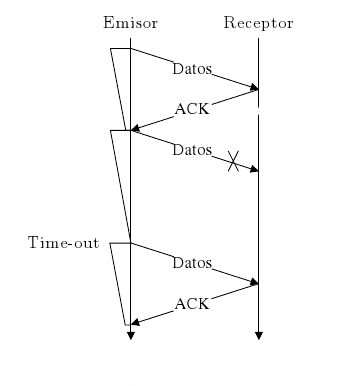
\includegraphics[width=0.5\linewidth]{sw_flow.png}
    \caption{Flujo básico SW con pérdida}
\end{figure}

Algunas decisiones de implementación tomadas que vale la pena aclarar:
\begin{itemize}
    \item \textbf{El número de ACK devuelto es el mismo al del paquete recibido}, no el siguiente como en otras implementaciones. Simplemente lo implementamos así desde el principio y no encontramos motivos para no mantenerlo de esta forma.
    \item \textbf{Basado en timeouts en vez de NAK}. Si bien conocemos que haciendo uso de NAK es probable observar una mejora en el tiempo total de transferencia más sobre un enlace con pérdida y retransmisiones, decidimos no tomar esta idea y simplemente mantener los timeouts. El motivo es porque consideramos más útil centrar nuestros esfuerzos en otros aspectos del trabajo y sabíamos que usando timeouts para el emisor de los paquetes ya manejamos tanto el caso base de uso de timeouts por pérdida de paquetes como la necesidad de retransmisión en caso de que el paquete esperado por el receptor no sea el enviado, probablemente mismo causado por la pérdida.
\end{itemize}

\subsection{Selective Repeat}
Explicar funcionamiento, arquitectura.

\subsection{Servidor}
En la solución implementada, la responsabilidad del servidor en sí es enfocada a la recepción de mensajes y manejo de clientes, en la siguiente \autoref{fig:server-a-rol} se puede observar un flujo común de comunicación entre un cliente y servidor

\begin{figure}[H]
    \centering
    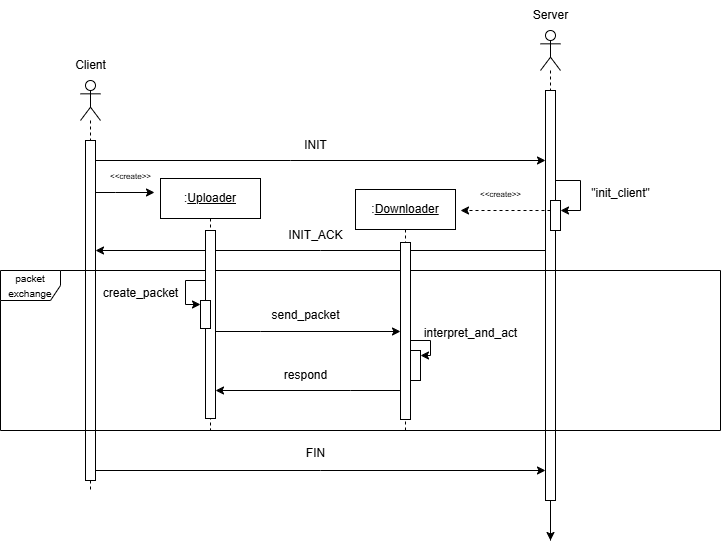
\includegraphics[width=0.5\linewidth]{client_server_exchange.png}
    \caption{Modelo de flujo de recepción de mensaje del servidor hacia procesamiento del mismo}
    \label{fig:server-a-rol}
\end{figure}

\textit{En la próxima sección documentaremos las entidades intermedias agregadas al diagrama de secuencia.}
El servidor entonces se encarga del manejo del socket con el que todos los clientes se comunican. A partir de la recepción de un mensaje, el flujo puede continuar:
\begin{enumerate}
        \item Si es el primer mensaje de un cliente, se procede a continuar el handshake, que consiste en enviar el INITACK y del punto de vista del servidor se considera la conexión establecida. Se agrega la conexión a la colección de conocidas y en caso de "download" por parte del cliente manda el/los paquetes necesarios a modo kickstart.
        \item Si el mensaje procede de una dirección de cliente conocida, se le pasa la información al proceso encargado de reaccionar a este y el flujo continua.
        \item Un caso particular, es la recepción de mensaje FIN por parte de un cliente, en este caso se cierra la conexión y liberan los recursos asociados al proceso con el cliente.
\end{enumerate}
Relacionado a la implementación, el hilo principal lee la información del socket y lanza un hilo por cada mensaje recibido para que pueda resolverse qué hacer con ese mensaje. Para el caso más interesante, que es el de transferencia de datos en si, le comunicamos al handler (explicado en la próxima sección) la información recibida mediante una Queue. Y haciendo, en caso que haya estado esperando, que se desbloquee su ejecución.

\subsection{Arquitectura enfocada en roles}
Como se pudo notar, por lo pronto no entramos en detalle con respecto a la implementación o arquitectura de la solución en ninguno de los sub-puntos. Esto se debe a que decidimos encarar la solución a partir de los roles que cada entidad asume, nosotros los llamamos Uploader y Downloader pero son análogos a Emisor y Receptor.
Como se comentó brevemente en la sección de Servidor, la responsabilidad propia del envío o recepción de mensajes se delega en el rol de la entidad en el traspaso de archivo. De esta forma, la responsabilidad de las entidades Cliente o Servidor se limitan a la iniciación y finalización de la comunicación y traspaso de información recibida del socket a la implementación del rol que asumen con la información comunicada en el mensaje INIT.

\subsection{Data \& Protocol Workers}
Para que la solución sea más performante decidimos "separar" la escritura y lectura de archivos del manejo de paquetes o procesos relacionados al protocolo. Para esto, las operaciones relacionadas a los archivos son "background", más específicamente es concurrente. Por ejemplo: en el caso de Uploader, un hilo está constantemente leyendo chunks de información del archivo a enviar a la otra entidad (de tamaño definido por el packet size a enviar) y carga esta información en una estructura de cola; a este proceso lo nombramos "data\_worker". Luego, el "protocol\_worker", es decir, el algoritmo encargado de efectivamente enviar esa información, toma la información de la cola, la paquetiza y envía según el protocolo utilizado.
De esta manera, reducimos el tiempo que toma enviar un mensaje realizando el proceso de forma secuencial y aprovechamos los "tiempos muertos" propios de la transmisión de información por una red (tenga o no packet loss). Además aseguramos la sincronización entre los procesos debido a la naturaleza bloqueante del Queue.Get() de Python. 

\section{Pruebas}
Se realizaron pruebas para comparar el rendimiento de los protocolos Stop \& Wait y Selective Repeat bajo distintas condiciones de pérdida de paquetes. Las pruebas incluyeron la transferencia de un archivo de 5.2MB simulando varios porcentajes de pérdida de paquetes (0\%, 10\%, y 20\%) utilizando Mininet para emular las condiciones de la red. Para verificar la integridad de los archivos transferidos, se realizo diff entre ambos archivos verificando que sean iguales. También se verificó en WireShark el tráfico generado, confirmando que los mensajes del protocolo seguían el formato definido.

\subsection*{Resultados}

\begin{itemize}
    \item Tiempos de transferencia para un archivo de 5.2MB con diferentes porcentajes de pérdida:
    \begin{itemize}
        \item \textbf{0\% Pérdida}:
        \begin{itemize}
            \item Selective Repeat (Upload): 2.39 segundos
            \item Selective Repeat (Download): 1.43 segundos
            \item Stop \& Wait (Upload): 4.91 segundos
            \item Stop \& Wait (Download): 4.12 segundos
        \end{itemize}
        \item \textbf{10\% Pérdida}:
        \begin{itemize}
            \item Selective Repeat (Upload): 91.16 segundos
            \item Selective Repeat (Download): 94.72 segundos
            \item Stop \& Wait (Upload): 85.67 segundos
            \item Stop \& Wait (Download): 82.33 segundos
        \end{itemize}
        \item \textbf{20\% Pérdida}:
        \begin{itemize}
            \item Selective Repeat (Upload): 213.62 segundos
            \item Selective Repeat (Download): 185.18 segundos
            \item Stop \& Wait (Upload): 200.48 segundos
            \item Stop \& Wait (Download): 200.97 segundos
        \end{itemize}
    \end{itemize}
\end{itemize}

\section{Preguntas a responder}
\subsection{Describa la arquitectura Cliente-Servidor}
La arquitectura Cliente-Servidor es un modelo de comunicación donde dos entidades principales interactúan: el cliente, que solicita servicios, y el servidor que los proporciona.

El cliente es el componente que inicia la comunicación. Su función es enviar solicitudes al servidor y recibir las respuestas adecuadas.

Por otro lado, el servidor gestiona y almacena los recursos solicitados, como bases de datos, archivos o aplicaciones. Este es quien escucha las solicitudes del cliente, las procesa y responde con la información solicitada.

La comunicación entre cliente y servidor se realiza mediante protocolos de red, siendo TCP/IP el más utilizado. Este conjunto garantiza que los datos lleguen de forma segura y ordenada. En entornos web, también se emplean protocolos como HTTP o HTTPS.

\subsection{¿Cuál es la función de un protocolo de capa de aplicación?}
La función de la capa de aplicación es permitir una comunicación eficaz y segura entre diferentes programas de aplicación dentro de una red. Para lograrlo, se utilizan protocolos específicos que definen cómo deben formatearse, enviarse, recibirse e interpretarse los mensajes entre aplicaciones.

Un protocolo de capa de aplicación establece las reglas que permiten que dos programas puedan intercambiar información correctamente, aunque estén en dispositivos distintos y en redes diferentes.

Además de facilitar la comunicación, estos protocolos aseguran que los datos lleguen de forma comprensible y estructurada.

\subsection{Detalle el protocolo de aplicación desarrollado en este trabajo}
Se explica en la sección de Implementación.

\subsection{La capa de transporte del stack TCP/IP ofrece dos protocolos: TCP y UDP. ¿Qué servicios proveen dichos protocolos? ¿Cuáles son sus características? ¿Cuándo es apropiado utilizar cada uno?}

\subsection*{TCP (Transmission Control Protocol)}

\begin{itemize}
    \item Proporciona una conexión confiable.
    \item Asegura la entrega completa, ordenada y sin duplicados de los datos.
    \item Realiza control de flujo y de congestión.
    \item Requiere el establecimiento de una conexión (handshake de tres pasos).
\end{itemize}

\textbf{Cuándo se utiliza:} cuando se necesita alta fiabilidad, como en:
\begin{itemize}
    \item Navegación web (HTTP/HTTPS)
    \item Transferencia de archivos (FTP)
    \item Correo electrónico
\end{itemize}

\subsection*{UDP (User Datagram Protocol)}

\begin{itemize}
    \item No orientado a la conexión (no requiere handshake).
    \item No garantiza entrega ni orden.
    \item Tiene menor sobrecarga y mayor velocidad que TCP.
    \item No realiza control de flujo ni de congestión.
\end{itemize}

\textbf{Cuándo se utiliza:} cuando se prioriza la velocidad sobre la fiabilidad, como en:
\begin{itemize}
    \item Video llamadas y streaming en vivo
    \item Consultas DNS
\end{itemize}


\section{Dificultades encontradas}
Las dificultades encontradas durante el proyecto incluyeron la definición de estructuras de mensajes, el manejo efectivo de timeouts, la lógica para la recuperación de pérdida de paquetes y la gestión de la ejecución concurrente en el servidor. El uso de concurrencia fue útil para manejar múltiples clientes, pero requiere un análisis cuidadoso para evitar posibles vulnerabilidades como el agotamiento de recursos.

\section{Conclusión}

La conclusión principal que obtenemos de este trabajo práctico es que efectivamente se logró crear un protocolo de transferencia de datos confiable (RDT) sobre UDP, un protocolo que por sí solo no ofrece garantías de fiabilidad. Esto se realizó mediante el desarrollo de una aplicación cliente-servidor orientada a la transferencia de archivos. Se implementaron dos mecanismos RDT sobre UDP: \textbf{Stop \& Wait} y \textbf{Selective Repeat }.

\begin{itemize}
    \item \textbf{Stop \& Wait (SW)} resultó ser más simple de implementar. Su lógica es directa, lo cual facilita su desarrollo y depuración. Es útil en redes con baja pérdida, aunque menos eficiente en términos de uso del canal.
    
    \item \textbf{Selective Repeat (SR)} tiene una implementación más compleja, dado que maneja ventanas deslizantes y múltiples paquetes en tránsito.

\end{itemize}

En las pruebas realizadas, ambos protocolos lograron cumplir su propósito fundamental: garantizar la llegada de los datos de forma confiable entre host y host, incluso en presencia de pérdidas de paquetes simuladas. Esto demuestra que, mediante un diseño adecuado en la capa de aplicación, es posible construir comunicación confiable sobre una base no confiable como UDP.

En definitiva, los protocolos desarrollados cumplieron con su objetivo: ofrecer un mecanismo robusto de transferencia de archivos, resaltando la importancia del protocolo de la capa de aplicación en garantizar la fiabilidad cuando la capa de transporte no lo hace.

\end{document}
